
\documentclass[11pt]{article}

    \usepackage{float}
    \usepackage{cleveref}
    \usepackage[T1]{fontenc}
    % Nicer default font than Computer Modern for most use cases
    \usepackage{palatino}
    \usepackage{listings}
    \usepackage{subcaption}

    % Basic figure setup, for now with no caption control since it's done
    % automatically by Pandoc (which extracts ![](path) syntax from Markdown).
    \usepackage{graphicx}
    % We will generate all images so they have a width \maxwidth. This means
    % that they will get their normal width if they fit onto the page, but
    % are scaled down if they would overflow the margins.
    %\setcounter{section}{-1}
    \makeatletter
    \def\maxwidth{\ifdim\Gin@nat@width>\linewidth\linewidth
    \else\Gin@nat@width\fi}
    \makeatother
    % \let\Oldincludegraphics\includegraphics
    % Set max figure width to be 80% of text width, for now hardcoded.
    % \renewcommand{\includegraphics}[1]{\Oldincludegraphics[width=.8\maxwidth]{#1}}
    % Ensure that by default, figures have no caption (until we provide a
    % proper Figure object with a Caption API and a way to capture that
    % in the conversion process - todo).
    % \usepackage{caption}
%    \DeclareCaptionLabelFormat{nolabel}{}
%    \captionsetup{labelformat=nolabel}

    \usepackage{adjustbox} % Used to constrain images to a maximum size
    \usepackage{xcolor} % Allow colors to be defined
    \usepackage{enumerate} % Needed for markdown enumerations to work
    \usepackage{geometry} % Used to adjust the document margins
    \usepackage{amsmath} % Equations
    \usepackage{amssymb} % Equations
    \usepackage{textcomp} % defines textquotesingle
    % Hack from http://tex.stackexchange.com/a/47451/13684:
    \AtBeginDocument{%
        \def\PYZsq{\textquotesingle}% Upright quotes in Pygmentized code
    }
    \usepackage{upquote} % Upright quotes for verbatim code
    \usepackage{eurosym} % defines \euro
    \usepackage[mathletters]{ucs} % Extended unicode (utf-8) support
    \usepackage[utf8x]{inputenc} % Allow utf-8 characters in the tex document
    \usepackage{fancyvrb} % verbatim replacement that allows latex
    \usepackage{grffile} % extends the file name processing of package graphics
                         % to support a larger range
    % The hyperref package gives us a pdf with properly built
    % internal navigation ('pdf bookmarks' for the table of contents,
    % internal cross-reference links, web links for URLs, etc.)
    \usepackage{hyperref}
    \usepackage{longtable} % longtable support required by pandoc >1.10
    \usepackage{booktabs}  % table support for pandoc > 1.12.2
    \usepackage[normalem]{ulem} % ulem is needed to support strikethroughs (\sout)
                                % normalem makes italics be italics, not underlines
                                
    \newcommand{\argmin}{\mathop{\rm arg\,min}\limits} % argmin command

    % Colors for the hyperref package
    \definecolor{urlcolor}{rgb}{0,.145,.698}
    \definecolor{linkcolor}{rgb}{.71,0.21,0.01}
    \definecolor{citecolor}{rgb}{.12,.54,.11}


    % Define a nice break command that doesn't care if a line doesn't already
    % exist.
    \def\br{\hspace*{\fill} \\* }
    % Math Jax compatability definitions
    \def\gt{>}
    \def\lt{<}
    % Document parameters
    \title{Non-negative Matrix Factorization in Application to Signal Denoising}


    % Exact colors from NB
    \definecolor{incolor}{rgb}{0.0, 0.0, 0.5}
    \definecolor{outcolor}{rgb}{0.545, 0.0, 0.0}


    % Prevent overflowing lines due to hard-to-break entities
    \sloppy
    % Setup hyperref package
    \hypersetup{
      breaklinks=true,  % so long urls are correctly broken across lines
      colorlinks=true,
      urlcolor=urlcolor,
      linkcolor=linkcolor,
      citecolor=citecolor,
      }
    % Slightly bigger margins than the latex defaults

    \geometry{verbose,tmargin=1in,bmargin=1in,lmargin=1in,rmargin=1in}



\begin{document}

\maketitle

\begin{figure}[H]
\centering
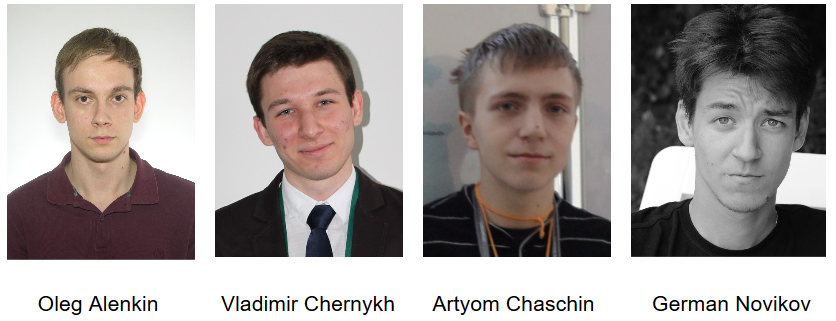
\includegraphics[width=1.\maxwidth]{team.png}
\end{figure}

\section{Spheres of responsibility}

\begin{table}[H]
\centering
%\caption{My caption}
\label{my-label}
\begin{tabular}{|l|l|}
\hline
\begin{tabular}[c]{@{}l@{}}Brainstorming, reading related articles\\ and literature, developing the common concept.\end{tabular}                        & All              \\ \hline
\begin{tabular}[c]{@{}l@{}}NMF algorithms analysis,\\ implementation of optimization methods, their comparison.\end{tabular}                               & Oleg, Artyom     \\ \hline
\begin{tabular}[c]{@{}l@{}}Building denoising pipeline - signal processing,\\ dictionaries construction, reconstruction of denoised signal.\end{tabular} & Vladimir, German \\ \hline
\end{tabular}
\end{table}

\section{Background}

Noisy speech signals are a common problem in many applications. For example, Automatic Speech Recognition (\textbf{ASR}). Machine understanding of what was said and how it was said is still far from humans. Well-developed methods of speech denoising will allow to improve different supporting systems dealing with speech processing like Siri, Yandex Maps etc. Speech denoising techniques may also be useful for increasing quality of telephone, skype and other types of conversations. One more possible application is hearing aids devices for people with auditory disabilities.

Recently, Non-negative Matrix Factorization (\textbf{NMF}) was successfully used for tackling this problem. Briefly, the idea is to use \textbf{NMF} to construct dictionaries of patterns for both clean speech signal and background noise. Then we can decompose any noisy signal into combination of basis vectors from both dictionaries and take only the components corresponding to clean part.

\section{Problem formulation}

The general formulation of the denoising problem is the following: we need to build transformation function $f: \mathbb{R}^{*} \mapsto \mathbb{R}^*$ (actually choose the best from some set $\mathcal{F}$) which maps the noisy signal into the clean one with the least possible error. Error can be expressed in many different ways in that case. Let's consider two of them:
\begin{itemize}
\item Signal error
\begin{gather*}
f^* = \argmin_{f \in \mathcal{F}}\|s_{clean} - f(s_{noisy})\|
\end{gather*}
It corresponds to the difference of the clean signal and reconstructed one.
\item Spectral error
\begin{gather*}
f^* = \argmin_{f \in \mathcal{F}}\|\text{STFT}\left(s_{clean}\right) - \text{STFT}\left(f(s_{noisy})\right)\|
\end{gather*}
In general the idea is the same - measure the error between the clean and reconstructed signal. But now the distance is calculated between their spectrograms.
\end{itemize}
In this work we're going to use the Spectral error because of the better robustness \cite{hu}.

To solve the problem of denoising, nonnegative matrix factorization (NMF) is frequently used (see section \ref{sec:solution} for the pipeline and the place of NMF in it). The goal of NMF is to decompose matrix $V \in \mathbb{R}^{n \times m}$ with nonnegative elements into product of two matrices $W \in \mathbb{R}^{n \times k}$ and $H \in \mathbb{R}^{k \times m}$ with nonnegative values and $k < \min(m,n)$, such that $V \approx W \cdot H$. In other words one should solve the following problem:
$$
W^*,H^* = \argmin_{W \geq 0, H \geq 0} D(V, WH),
$$
where $D(V, WH)$ is a “distance” between two matrices. Various functions are used for $D$, which leads to different problems and different solutions for them. 

The common choice here is to use so called \textit{separable} distance that is when $D(P, Q)$ can be decomposed into elementwise computations. The advantage of such functions is that computations proceed much faster than with usual matrix norms and saved time can be used to do multistart which is much more useful regarding the multiextremality of the problem. In our work we use two following distances:
\begin{itemize}
\item Kullback–Leibler divergence
\begin{gather*}
D_{KL}(P,Q) = \sum_{i,j = 1}^{n}d(p_{ij}, q_{ij}), \\
d(p, q) = p \ln \frac{p}{q} − p + q.
\end{gather*}
\item Frobenius norm of matrices difference
\begin{gather*}
D_{KL}(P,Q) = \|P - Q\|_{F}
\end{gather*}
\end{itemize}
Also we try to use the regularization to preserve the sparseness of the matrix $H$ which should increase the quality of the solution \cite{cauchi}. For that purpose we use L1-norm and following objective function:
\begin{gather*}
D_{KL}(P,Q) = \|P - Q\|_{F} + \lambda \|H\|_1
\end{gather*}

\section{Solution} \label{sec:solution}

Our solution has two more or less distinct parts: general training and denoising workflow and NMF optimization problem.

\subsection{Denoising workflow}

In our project we came up with the following pipeline depicted at the figure \ref{fig:pipeline}
\begin{figure}[H]
\centering
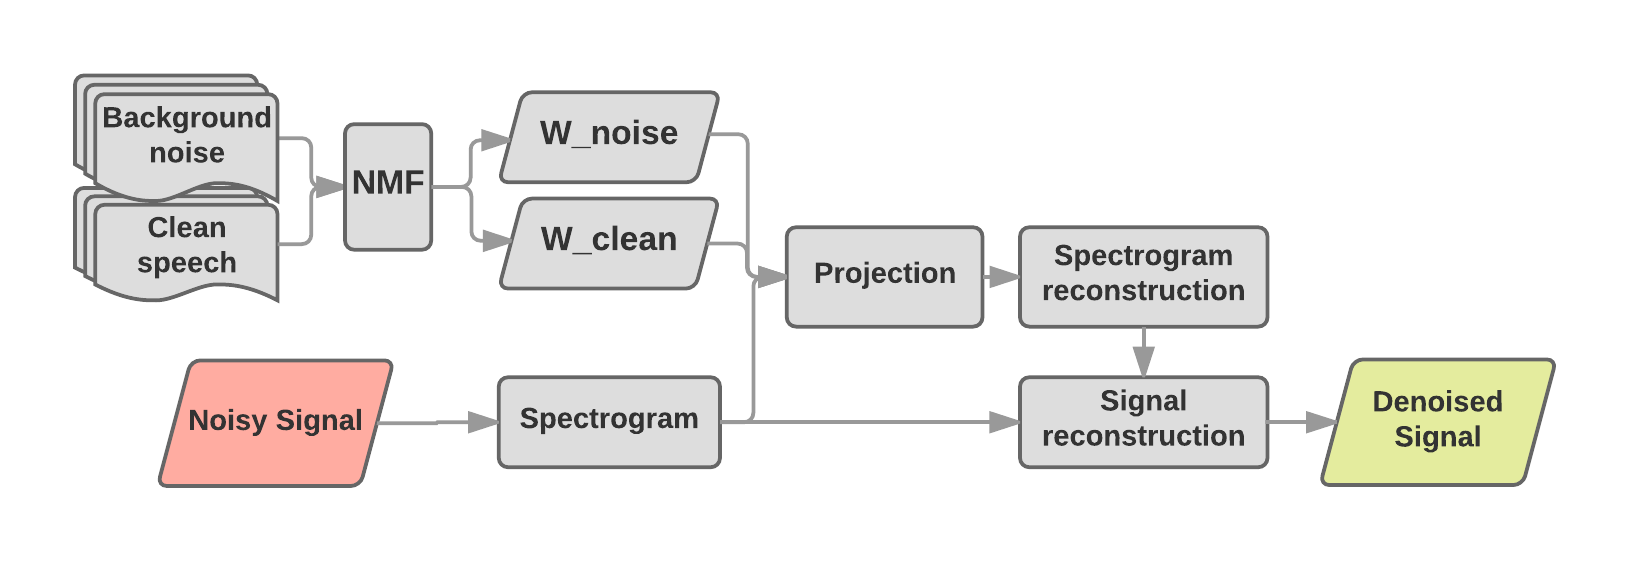
\includegraphics[width=1.\maxwidth]{solution.png}
\caption{Algorithm workflow}
\label{fig:pipeline}
\end{figure}

Let’s briefly describe all the steps of the training stage:
\begin{itemize}
  \item Having background noise $s_{noise}$ and clean speech $s_{clean}$ we obtain their spectrograms $S_{noise}$ and $S_{clean}$. This is done by means of the Short-Term Fourier Transform that simply slides window across the signal and does usual FFT inside it. For more details on window selection see \href{https://github.com/elejke/CNMF-ASR/blob/master/code/Denoising_Demo.ipynb}{this piece} of the code in the format of IPython Notebook which follows the guidelines from \href{https://ccrma.stanford.edu/~jos/parshl/Choice_Hop_Size.html}{this} Stanford course.
  \item Working with complex spectrograms is not convenient, thus we want to obtain a real matrix from it. So we took the absolute values of each cell which corresponds to the magnitude matrix of the initial spectrogram. In that way we obtain $V_{clean} = |S_{clean}|$, $V_{noise} = |S_{noise}|$.
  \item After that we apply NMF to represent the magnitude matrices $V$ as a product of two nonnegative matrices $W$ and $H$. The interpretation of these matrices is the following: $W$ contains frequency “building blocks” or patterns of a signal, while $H$ contains time-activation information about it - when and how strong each pattern should be applied to form the initial signal in the best way. The intuitive toy example with the piano notes sequence can also be found in the \href{https://github.com/elejke/CNMF-ASR/blob/master/code/Piano_Example.ipynb}{code} (the idea is taken from \cite{smaragdis}).
  \item Through the NMF we learn dictionaries for both clean speech and background noise. The important thing to mention here is the hidden dimension (rank) of the NMF. Rank of decomposition for the clean speech is chosen approximately equal to the number of phonemes (distinct "building blocks" of speech) in the English language which is about 40.
\end{itemize}
The denoising stage then is the following:
\begin{itemize}
  \item Take the spectrogram of the noisy signal
  \item Project it on the already learned and joined vocabularies of clean and noise patterns - $W_{joined} = \begin{pmatrix} W_{clean} & W_{noise} \end{pmatrix}$. One can see the scheme in the figure \ref{fig:denoising} It is done by means of the subroutine of ANLS algorithm where one matrix ($W$ in this case) is fixed. Then we take only the “clean” component of this decomposition and our denoised magnitudes are $V_{reconstructed} = W_{clean}H_{joined}^{1:r_{clean}}$.
\begin{figure}[H]
\centering
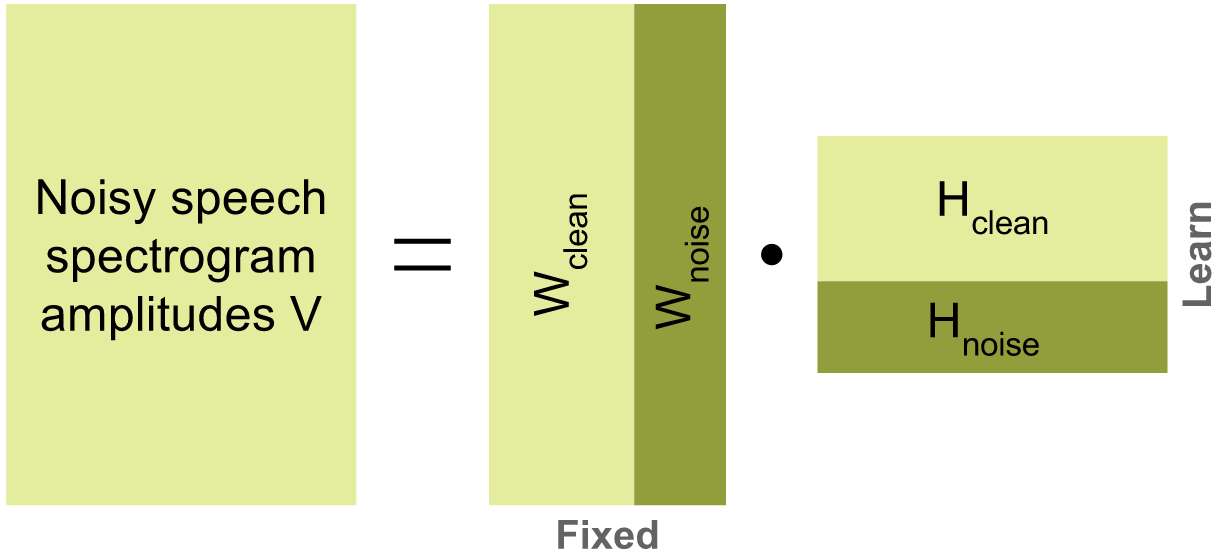
\includegraphics[width=0.9\maxwidth]{denoising_stage.png}
\caption{Denoising stage}
\label{fig:denoising}
\end{figure}
  \item The important step here is how to reconstruct the phase information from the magnitudes. This problem is quite complicated and there are few approaches invented for it \cite{griffin, sturmel}. In general case it is impossible to reconstruct the signal precisely. But we choose window parameters in such a way that they overlaps massively and thus implicitly store information about a phase. So reconstruction is possible and can be made in a few different ways which are described in details in our \href{https://github.com/elejke/CNMF-ASR/blob/master/code/Denoising_Demo.ipynb}{IPython Notebook}.
  \item The final step is to reconstruct the signal itself from the spectrogram. It is done by means of usual Inverse Short-Term Fourier Transformation.
\end{itemize}

\subsection{NMF problem}

The following methods for NMF were implemented:
\begin{itemize}
\item Multiplicative Update (MU) method with both KL divergence and Frobenius norm (we used the Nimfa library \cite{nimfa} for that).

MU is a kind of gradient descent. On each iteration we choose such step that vector $\mathbf{h}$ updates multiplicative. We divide gradient on positive and negative part. On each iteration we multiply our vector on $\frac{[\nabla_H^-]_{kj}}{[\nabla_H^+]_{kj}}$:
$$[\nabla_H]_{kj}=\frac{\partial D\left(V, WH\right)}{\partial h_{kj}}=[\nabla_H^+]_{kj}-[\nabla_H^-]_{kj}$$
$$h_{kj}\leftarrow h_{kj}-\frac{h_{kj}}{[\nabla_H^+]_{kj}}([\nabla_H^+]_{kj}-[\nabla_H^-]_{kj})=\frac{[\nabla_H^-]_{kj}}{[\nabla_H^+]_{kj}}h_{kj}$$

This approach allows us not to think about non-negativity of matrices $W$ and $H$, if they initialized as non-negative matrices, they can't become negative in process of descent.
\item Alternating Nonnegative Least Squares (ANLS) with Frobenius norm.

Structure of the algorithm is the following:

1) Initialize $W_{ia}^1 \geq 0$, $W_{bj}^1 \geq 0, \forall a,i,b,j$.

2) For $k=1,2,\dots$

$$W^{k+1}=\argmin_{W\geq 0}D\left(V, WH^{k} \right)$$
$$H^{k+1}=\argmin_{H\geq 0}D\left(V, W^{k}H \right)$$

For solving subproblem we used projected gradient method.

\item ANLS Frobenius norm and L1 regularization of the matrix $H$.

The concept is the same but loss function is a bit changed.
$$W^*,H^* = \argmin_{W \geq 0, H \geq 0} \left( \|V- WH\|_F^2 + \lambda\|H\|_1 \right)$$

This method was already implemented in sklearn, also we tried to use CVX to solve the subproblem.
\item Quasi-Newton \cite{zdunek} method for KL divergence.

Probably the only method of second-order.

On each iteration we should do the following updates:

$$W\leftarrow \max(\varepsilon, W-H_W^{-1}\nabla_WD_{KL})$$
$$H\leftarrow \max(\varepsilon, H-H_H^{-1}\nabla_HD_{KL})$$

Where $H_W$ and $H_H$ are hessians. The main disadvantage of this method is hessian inversion. Hessian calculation described in details in \cite{zdunek}.
\end{itemize}

\section{Data}

We used \href{http://spandh.dcs.shef.ac.uk/chime_challenge/chime_download.html}{CHiME} dataset to test our algorithms. It contains different structural parts which are:
\begin{itemize}
  \item Clean segmented speech consisted of WSJ (Wall Street Journal) utterances recorded at the booth. The mean length if the utterance is about 5 seconds and the number of utterances is about 8000 from 4 different speakers.
  \item Background noise of 4 different types:
    \begin{itemize}
        \item Cafe
        \item Street
        \item Bus
        \item Pedestrian area
    \end{itemize}
  \item Noisy speech which was obtained by corrupting the initial clean data via \href{http://aurora.hsnr.de/download.html}{Aurora} and described background noise.
\end{itemize}

\section{Related works}

There were many tries to apply NMF for speech denoising \cite{cauchi, lyubimov, smaragdis, wilson, vaz}. All of them uses slightly different ways of doing NMF, which will be covered later in this section. But one more significant difference between all works which virtually divides them into two non-overlapping classes - way of denoising. Here we also include third type of methods to fully cover all the denosing ways (not only with NMF)
\begin{itemize}
\item \textit{Unsupervised}. This paradigm requires no additional data like background noise or clean speech is available. The successful examples of this approach are Minimum Mean Squared Error estimator \cite{ephraim} and Spectral Subtraction \cite{boll}
\item \textit{Semi-supervised}. In their papers \cite{cauchi, lyubimov} authors assume the availability only of the background noise signals at the training stage. Their pipeline implies pre-train dictionary only for the noise and then try to extract noise part from the noisy speech.
\item \textit{Supervised}. In this approach \cite{wilson, vaz} the assumption is that we have both background noise and clean speech at the training stage. Then one can come up with the pipeline described in section \ref{sec:solution}.
\end{itemize}

The main concept of NMF denoising is to reject components corresponding to noise from the signal. Several approaches were considered earlier.

A lot of researchers developing new methods for NMF use Multiplicative Updates method as a baseline solution \cite{riab}. It is one of the first and simplest method. The most actively used method today is Alternating Non-negative Least Squares \cite{riab}. Second-order methods are not common for NMF problem due to both their computational complexity and usually big dimension problems in NMF applications. Nevertheless at least one method has been developed \cite{zdunek}.

Also sparseness of decomposition may be benefitial for the denoising problem. It was shown that somtimes  it is a good idea to use regularization \cite{cauchi} to provide sparseness of coefficient matrix $H$.

\section{Scope}

The initial plan was to implement all the stages of signal denoising by ourselves. First, we wanted to implement the part responsible for signal processing: spectrogram generation, construction of clean and noisy dictionaries, signal decomposition into combination of noisy and clean basis vectors. Also we wanted to get acquainted with popular methods of NMF, some of them were already implemented \cite{nimfa}, some were assumed to be implemented by ourselves. Briefly, the aim of this work was to get positive result, check that this approach is able to denoise signal significantly.

\section{Evaluation}

The performance of our solution (NMF part) is measured by the distance between the original matrix and the product of two generated matrices $D(V, WH)$. As mentioned before, we used KL divergence and Frobenius norm as a distance function.

For measuring the quality of the signal reconstruction there are several ways (see \cite{hu} for further details):
\begin{itemize}
  \item Distance between clean and denoised signals. The drawback of this method is that reconstructed signal may be of a very good quality but signals can greatly varies due to the little phase shifts during the reconstruction.
  \item “Spectral distance“ - matrix distance between spectrograms of clean signal and denoised one. This metric is more robust than the previous one.
  \item Signal-to-Noise-Ratio (SNR) - ratio of the “useful” signal containing in the signal to the noise containing into it. This metric requires to have signals normed and thus we didn’t use it.
\end{itemize}
    
\section{Results}

As a result of our work we implement the proposed workflow for the speech denoising. One of the unexpected difficulties was the part with the signal reconstruction from the magnitudes because we don't think about it at the beginning of the project. But when we faced this problem we brainstormed the possible solutions, investigate the papers on this topic and come up with a few solutions comparison of which can also be found in \href{https://github.com/elejke/CNMF-ASR/blob/master/code/Denoising_Demo.ipynb}{IPython notebook}.

\subsection{NMF}

In the figure \ref{fig:NMFoptimization} one can observe the convergence of all 4 tested optimization methods. In the figure \ref{fig:frob} there are three algorithms compared in terms of Frobenius norm of difference of a matrix $\|V - W \cdot H\|_{F}$: ANLS with Frobenius norm, MU with Forbenius norm, ANLS with Frobenius + L1-regularization. While in the figure \ref{fig:kl} we compare the same ANLS algorithms (ANLS with Frobenius norm and ANLS with Frobenius + L1-regularization) but MU algorithm now minimizes the KL divergence.

\begin{figure}[H]
	\begin{subfigure}{.5\textwidth}
		\centering
		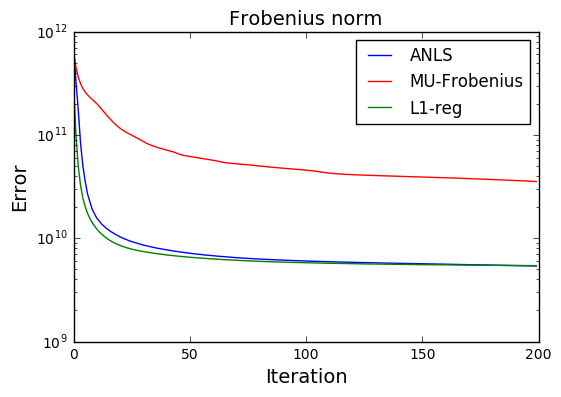
\includegraphics[width=1.0\linewidth]{gr1.png}
		\caption{Frobenius norm}
		\label{fig:frob}
	\end{subfigure}
	\begin{subfigure}{.5\textwidth}
		\centering
		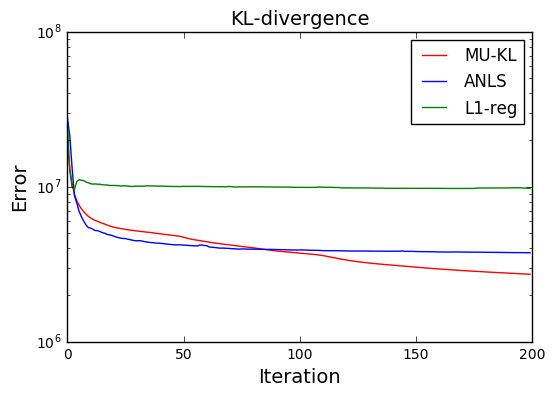
\includegraphics[width=1.0\linewidth]{gr2.png}
		\caption{KL divergence}
		\label{fig:kl}
	\end{subfigure}
	\caption{Comparison of NMF optimization algorithms in different norms}
	\label{fig:NMFoptimization}
\end{figure}

In terms of both KL divergence and Frobenius norm our implementation of ANLS shows good result. So, we decided to use ANLS in final version of the pipeline.

As for Quasi-Newton method, we implemented it, but didn’t apply it to the magnitudes matrix $V$ explicitly, because it needs a lot of resources (actually we ran out of memory with the spectrograms). Demonstration of the algorithm on smaller matrices can be found in separate \href{https://github.com/elejke/CNMF-ASR/blob/master/code/Quasi_Newton_Demo.ipynb}{notebook}. So as it was mentioned before, methods of the second order are not the best way to deal with the NMF, it is much better to use any gradient methods with multistart, moreover problem is multiextremal.

\subsection{Denoising}

During the denoising stage we used 4 different algorithms for reconstruction of the signal. In the figure \ref{fig:iterative} one can see how well denoised signal approximates the clean one.
\begin{figure}[H]
\centering
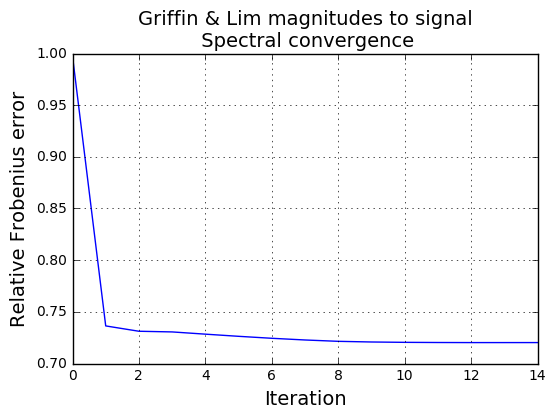
\includegraphics[width=0.5\maxwidth]{griffin&lim.png}
\caption{Spectral convergence of iterative reconstruction method}
\label{fig:iterative}
\end{figure}
While quantitative results are not very impressive, it's much better if we compare audio signals judging on their sounding and looking at the spectrograms with eyes. Audio signals can be found in the \href{https://github.com/elejke/CNMF-ASR/blob/master/code/Denoising_Demo.ipynb}{IPython Notebook}.

For the visual comparison, consider figure \ref{fig:comparison} where one can observe raw data and their spectrograms for three signals: clean speech, noisy speech and denoised one via proposed framework.

\begin{figure}[H]
\centering
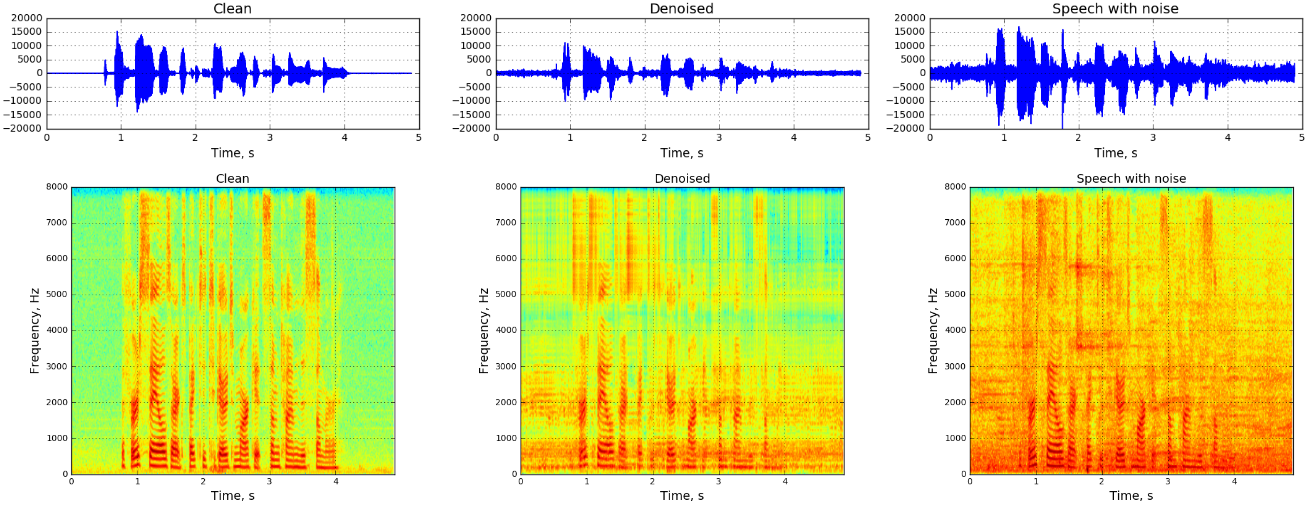
\includegraphics[width=1.\maxwidth]{spectrograms.png}
\caption{Comparison of clean, denoised and noisy signals}
\label{fig:comparison}
\end{figure}

From this comparison one can notice significant bias of the denoised signal towards the clean one.

\section{Conclusion and Future Work}

In this work we implemented the full process of signal denoising. We analyzed different iterative methods of non-negative matrix factorization and compared them with each other. Concept of decomposition the signal into combination of basis vectors from two dictionaries was used. Also we faced with problem of reconstruction signal from its spectrogram magnitudes. We came up with the algorithm which is able to clean most part of the noisy signal. Some work may be done in the direction of regularized optimization problem, because it didn't give anticipated improvement reported in other papers.

During the work process and development of the initial idea we also found out that researchers \cite{vaz, ogrady} try to use Convolutive NMF to deal with the denoising problem. This idea sounds perspective from our point of view because of the two reasons: speech itself has a time-continual structure and applying convolutions here looks more than reasonable; recently many deep learning approaches for speech recognition and generation (e.g. amazing \href{https://deepmind.com/blog/wavenet-generative-model-raw-audio/}{Google Wavenet}) rely on convolutions in their architectures and is able show state-of-the-art performance in virtue of that. So the next step of our research may be to embed CNMF into our framework.

\begin{thebibliography}{99}
\addcontentsline{toc}{section}{Literature}

\bibitem{cauchi} Cauchi B., Goetze S., Doclo S. (2012). \textit{Reduction of Non-stationary Noise for a Robotic Living Assistant using Sparse Non-negative Matrix Factorization}.

\bibitem{griffin} Griffin D. W., Lim J.S. (1984). \textit{Signal  Estimation  from  Modified  Short-Time Fourier  Transform}. IEEE Transactions On Acoustics, Speech, And Signal Processing,  Vol. ASSP-32, No. 2, April 1984

\bibitem{hu} Hu Y., Loizou P. C. (2008). \textit{Evaluation of Objective Quality Measures
for Speech Enhancement}. IEEE Transactions On Audio, Speech, And Language Processing,  Vol. 16, No. 1, January 2008

\bibitem{lyubimov} Lyubimov N., Kotov M. (2013). \textit{Non-negative Matrix Factorization with Linear Constraints for Single-Channel Speech Enhancement}.

\bibitem{nimfa} Nimfa, a Python library for nonnegative matrix factorization. http://nimfa.biolab.si/

\bibitem{smaragdis} Smaragdis P. (2005) \textit{From Learning Music to Learning to Separate}. Forum Acusticum Budapest 2005: 4th European Congress on Acoustics. (pp. 1545-1549)

\bibitem{sturmel} Sturmel N., Daudet L. (2011). \textit{Signal Reconstruction from STFT Magnitude: A State-of-the-Art}. Proc. of the 14th Int. Conference on Digital Audio Effects (DAFx-11), Paris, France, September 19-23, 2011

\bibitem{wilson} Wilson K. W., Raj B., Smaragdis P., Divakaran A. (2008). \textit{Speech denoising using nonnegative matrix factorization with priors}.

\bibitem{zdunek} Zdunek R., Cichocki A. (2006). \textit{Non-Negative Matrix Factorization with Quasi-Newton Optimization}. Eighth International Conference on Artificial Intelligence and Soft Computing, ICAISC, pages 870–879

\bibitem{vaz} Vaz C., Dimitriadis D., Thomas S., Narayanan S. (2016) \textit{CNMF-based Acoustic Features for Noise-Robust ASR}. Proceedings of IEEE International Conference on Audio, Speech and Signal Processing (ICASSP), Shanghai, China, 2016.

\bibitem{riab} Riabenko E. A. (2014). \textit{Loss function choice in problem of non-negative matrix factorization}.

\bibitem{ogrady} O’Grady P.D., Pearlmutter B.A. (2006) \textit{Convolutive non-negative matrix factorisation with a sparseness constraint}. In Proc. of the 2006 16th IEEE Signal Processing Society Workshop on Machine Learning for Signal Processing, pages 427–432.

\bibitem{ephraim} Ephraim Y., Malah D. (1984) \textit{Speech enhancement using a minimum mean square error short-time spectral amplitude estimator}. IEEE Transactions on Acoustic, Speech and Signal Processing, 32(6):1109–1121, 1984

\bibitem{boll}  Boll S. (1979) \textit{Suppression of acoustic noise in speech using spectral subtraction}. IEEE Transactions on Acoustics Speech and Signal Processing,
27(2):113–120, 1979

\end{thebibliography}{}

\end{document}
